\newpage
\section*{9\quad Inference: the KV cache and its bill}
\addcontentsline{toc}{section}{9 Inference: the KV cache}
\startchapter{9}
\providecommand{\fitR}[1]{\leavevmode\setbox0\hbox{#1}\ifdim\wd0>\linewidth\resizebox{\linewidth}{!}{\box0}\else\box0\fi}

\begin{chaptermap}
Up to now we have trained the model to answer $T$ exercises in one pass. Using it is a different job: the
reply is written one token at a time, and each new token has to wait for the one before it. This chapter
asks what that loop costs. We find that most of the work in it is repeated, we remove the repetition with
the \emph{KV cache}, and we prove on the toy that the answer does not change by a single digit. Then we
count the bill the cache brings with it, in real gigabytes for GPT-2 and Qwen3, and look at two ideas that
shrink it: sharing keys and values between heads, and never writing the big score table to memory. It ends
with you able to price the memory of any model's conversation from its configuration.
\end{chaptermap}

\machine{9}{You are here: the \emph{KV cache} box, on the right of attention. It is not a new layer and it
changes no answer. It is a store next to every attention block that keeps the keys and values of the tokens
already read, so that writing the next token does not redo their work.}

\begin{beforeyoustart}
\begin{enumerate}[label=\arabic*.,leftmargin=1.6em]
\item How many bytes are in a kibibyte (KiB), a mebibyte (MiB) and a gibibyte (GiB)?
\item A number stored in ``fp16'' takes 16 bits. How many bytes is that?
\item What is $12 \times 64$? What is $2 \times 28 \times 8 \times 128$?
\item From Chapter 3: which of $Q$, $K$, $V$ does a token use to \emph{ask}, and which two does it use to
\emph{be found} and to \emph{hand over}?
\end{enumerate}
\textit{Refreshers.} (1) Computers count memory in powers of two: 1 KiB $= 1024$ bytes, 1 MiB $= 1024$ KiB,
1 GiB $= 1024$ MiB $= 2^{30} \approx 1.07$ billion bytes. (2) 8 bits make a byte, so fp16 is 2 bytes.
(3) 768 and 57{,}344. (4) The query asks; the key is what it can be found by; the value is what it hands
over. If any of these felt shaky, reread \S3.5 before going on.
\end{beforeyoustart}

%---------------------------------------------------------------------
\subsection*{9.1\quad Back to the loop}

Chapter 1 drew the loop that writes a reply: read the words so far, guess the next word, append it,
repeat. Our customer wrote \tok{waste of time}. To write \emph{Sorry, this has not been useful} the
model goes round the loop \nNineSteps\ times, and after the last turn the sequence is \nNineFinalT\ tokens long.

\Predict When the model writes the 8th token, it has already processed the first 7 tokens on earlier
turns. Tell me: how much of the work for those 7 tokens do you expect to be done \emph{again}? None, a
little, or almost all of it? Write down your guess before reading on.

\Picture Imagine keeping a diary where, every evening, before writing today's line, you copy out every
earlier page by hand and then add one sentence. Nothing on the old pages has changed. You are paying again
for work you already did.

\Summary{Writing is a loop, one token per turn, and each turn sees a longer sequence than the last.}

%---------------------------------------------------------------------
\subsection*{9.2\quad What gets repeated}

Let us count it on the toy instead of guessing. Take the attention of Chapter 3 and suppose that on every
turn we run it on the whole sequence so far, exactly as during training. For a sequence of $t$ tokens that
means making $t$ queries, $t$ keys and $t$ values ($3 \times t \times d \times d_k$ multiplications), then
the $t \times t$ score table, then mixing the values ($2 \times t \times t \times d_k$ more).

Now look at what is new on each turn. Only one token arrived. Its key and value are new, and its question
is new. Every earlier token's key and value are the same numbers they were last turn, because a token's
key is $\bm{x}W_K$ and neither its arrow nor $W_K$ has changed. And thanks to the causal mask (\S3.6, Step 3)
the earlier tokens' outputs cannot change either: they are not allowed to look at the newcomer.

\begin{center}
\small
\begin{tabular}{@{}r l r r@{}}
\toprule
length $t$ & newest token & multiplications, recompute all & multiplications, only the new token\\
\midrule
\nNineTable
\bottomrule
\end{tabular}
\end{center}

Over the \nNineSteps\ turns (plus reading the prompt once) that is \nNineMultFull\ multiplications for
recomputing everything against \nNineMultCache\ if we only compute what is new: \nNineRatio\ times less work,
on a reply of seven tokens. Notice how the left column grows: the score table part grows with $t^2$, so for a
reply of a thousand tokens the waste is far worse.

\begin{wrongidea}{9.1}
``Writing each new token means running the whole sentence through the model again.'' It is tempting because
the model does \emph{read} its whole context every turn. But reading is not recomputing. The new token needs
the old tokens' keys and values, and those were already computed on earlier turns. What has to be recomputed
is only what depends on the new token.
\end{wrongidea}

\Summary{On every turn, everything about the old tokens is the same as last turn; only the newest token brings
new work.}

%---------------------------------------------------------------------
\subsection*{9.3\quad The KV cache}

\Picture A librarian files a card for each book as it arrives: its label and a summary. When a new reader
comes with a question, the librarian does not reprint every card; they read through the existing cards with
the new question. Each new book adds one card.

\Exactly Keep two growing tables, $K_{\text{cache}}$ and $V_{\text{cache}}$, one row per token so far.
On each turn, for the newest token $\bm{x}_t$:
\[
\bm{q}_t = \bm{x}_t W_Q,\quad
K_{\text{cache}} \leftarrow \begin{bmatrix} K_{\text{cache}} \\ \bm{x}_t W_K \end{bmatrix},\quad
V_{\text{cache}} \leftarrow \begin{bmatrix} V_{\text{cache}} \\ \bm{x}_t W_V \end{bmatrix}
\shape{1\times d_k,\ t\times d_k,\ t\times d_k}
\]
\[
\bm{o}_t = \softmax\!\left(\frac{\bm{q}_t K_{\text{cache}}^\top}{\sqrt{d_k}}\right) V_{\text{cache}}
\shape{(1\times t)(t\times d_k) = 1\times d_k}
\]
One query row meets every cached key: one row of the tournament table, not the whole table.
Figure~\ref{fig:ch9grow} shows the two tables on our toy as the reply starts. Each turn adds one row at
the bottom (highlighted) and leaves every row above it untouched.

\begin{figure}[!tbp]
\centering
\fitR{% AUTO-GENERATED by code/figlib.py helpers -- do not edit
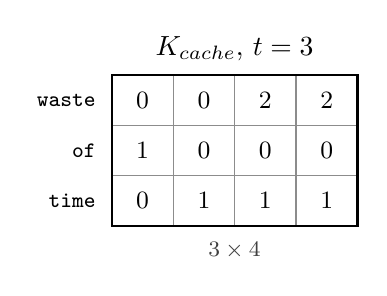
\begin{tikzpicture}
\draw[black!45, fill=white] (0.000,0.000) rectangle (0.780,-0.640);
\node[font=\small, text=black] at (0.390,-0.320) {$0$};
\draw[black!45, fill=white] (0.780,0.000) rectangle (1.560,-0.640);
\node[font=\small, text=black] at (1.170,-0.320) {$0$};
\draw[black!45, fill=white] (1.560,0.000) rectangle (2.340,-0.640);
\node[font=\small, text=black] at (1.950,-0.320) {$2$};
\draw[black!45, fill=white] (2.340,0.000) rectangle (3.120,-0.640);
\node[font=\small, text=black] at (2.730,-0.320) {$2$};
\draw[black!45, fill=white] (0.000,-0.640) rectangle (0.780,-1.279);
\node[font=\small, text=black] at (0.390,-0.959) {$1$};
\draw[black!45, fill=white] (0.780,-0.640) rectangle (1.560,-1.279);
\node[font=\small, text=black] at (1.170,-0.959) {$0$};
\draw[black!45, fill=white] (1.560,-0.640) rectangle (2.340,-1.279);
\node[font=\small, text=black] at (1.950,-0.959) {$0$};
\draw[black!45, fill=white] (2.340,-0.640) rectangle (3.120,-1.279);
\node[font=\small, text=black] at (2.730,-0.959) {$0$};
\draw[black!45, fill=white] (0.000,-1.279) rectangle (0.780,-1.919);
\node[font=\small, text=black] at (0.390,-1.599) {$0$};
\draw[black!45, fill=white] (0.780,-1.279) rectangle (1.560,-1.919);
\node[font=\small, text=black] at (1.170,-1.599) {$1$};
\draw[black!45, fill=white] (1.560,-1.279) rectangle (2.340,-1.919);
\node[font=\small, text=black] at (1.950,-1.599) {$1$};
\draw[black!45, fill=white] (2.340,-1.279) rectangle (3.120,-1.919);
\node[font=\small, text=black] at (2.730,-1.599) {$1$};
\draw[line width=0.9pt] (0.000,0.000) rectangle (3.120,-1.919);
\node[anchor=east, font=\footnotesize\ttfamily] at (-0.080,-0.320) {waste};
\node[anchor=east, font=\footnotesize\ttfamily] at (-0.080,-0.959) {of};
\node[anchor=east, font=\footnotesize\ttfamily] at (-0.080,-1.599) {time};
\node[anchor=south, font=\normalsize] at (1.560,0.050) {$K_{\text{cache}}$, $t=3$};
\node[anchor=north, font=\footnotesize, text=black!75] at (1.560,-1.999) {$3\times4$};
\end{tikzpicture}
\qquad
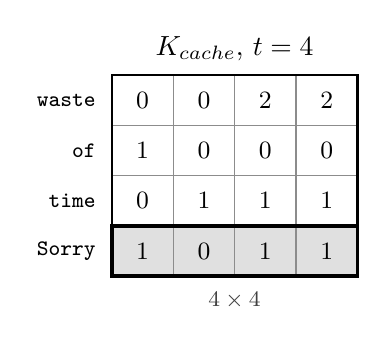
\begin{tikzpicture}
\draw[black!45, fill=white] (0.000,0.000) rectangle (0.780,-0.640);
\node[font=\small, text=black] at (0.390,-0.320) {$0$};
\draw[black!45, fill=white] (0.780,0.000) rectangle (1.560,-0.640);
\node[font=\small, text=black] at (1.170,-0.320) {$0$};
\draw[black!45, fill=white] (1.560,0.000) rectangle (2.340,-0.640);
\node[font=\small, text=black] at (1.950,-0.320) {$2$};
\draw[black!45, fill=white] (2.340,0.000) rectangle (3.120,-0.640);
\node[font=\small, text=black] at (2.730,-0.320) {$2$};
\draw[black!45, fill=white] (0.000,-0.640) rectangle (0.780,-1.279);
\node[font=\small, text=black] at (0.390,-0.959) {$1$};
\draw[black!45, fill=white] (0.780,-0.640) rectangle (1.560,-1.279);
\node[font=\small, text=black] at (1.170,-0.959) {$0$};
\draw[black!45, fill=white] (1.560,-0.640) rectangle (2.340,-1.279);
\node[font=\small, text=black] at (1.950,-0.959) {$0$};
\draw[black!45, fill=white] (2.340,-0.640) rectangle (3.120,-1.279);
\node[font=\small, text=black] at (2.730,-0.959) {$0$};
\draw[black!45, fill=white] (0.000,-1.279) rectangle (0.780,-1.919);
\node[font=\small, text=black] at (0.390,-1.599) {$0$};
\draw[black!45, fill=white] (0.780,-1.279) rectangle (1.560,-1.919);
\node[font=\small, text=black] at (1.170,-1.599) {$1$};
\draw[black!45, fill=white] (1.560,-1.279) rectangle (2.340,-1.919);
\node[font=\small, text=black] at (1.950,-1.599) {$1$};
\draw[black!45, fill=white] (2.340,-1.279) rectangle (3.120,-1.919);
\node[font=\small, text=black] at (2.730,-1.599) {$1$};
\draw[black!45, fill=black!12] (0.000,-1.919) rectangle (0.780,-2.558);
\node[font=\small, text=black] at (0.390,-2.239) {$1$};
\draw[black!45, fill=black!12] (0.780,-1.919) rectangle (1.560,-2.558);
\node[font=\small, text=black] at (1.170,-2.239) {$0$};
\draw[black!45, fill=black!12] (1.560,-1.919) rectangle (2.340,-2.558);
\node[font=\small, text=black] at (1.950,-2.239) {$1$};
\draw[black!45, fill=black!12] (2.340,-1.919) rectangle (3.120,-2.558);
\node[font=\small, text=black] at (2.730,-2.239) {$1$};
\draw[line width=1.4pt] (0.000,-1.919) rectangle (3.120,-2.558);
\draw[line width=0.9pt] (0.000,0.000) rectangle (3.120,-2.558);
\node[anchor=east, font=\footnotesize\ttfamily] at (-0.080,-0.320) {waste};
\node[anchor=east, font=\footnotesize\ttfamily] at (-0.080,-0.959) {of};
\node[anchor=east, font=\footnotesize\ttfamily] at (-0.080,-1.599) {time};
\node[anchor=east, font=\footnotesize\ttfamily] at (-0.080,-2.239) {Sorry};
\node[anchor=south, font=\normalsize] at (1.560,0.050) {$K_{\text{cache}}$, $t=4$};
\node[anchor=north, font=\footnotesize, text=black!75] at (1.560,-2.638) {$4\times4$};
\end{tikzpicture}
\qquad
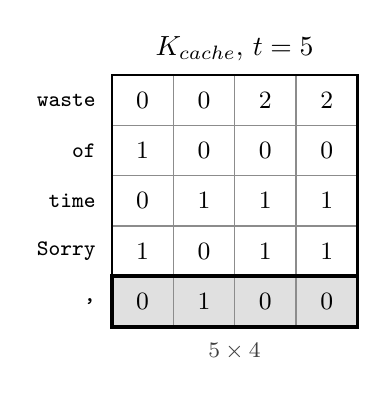
\begin{tikzpicture}
\draw[black!45, fill=white] (0.000,0.000) rectangle (0.780,-0.640);
\node[font=\small, text=black] at (0.390,-0.320) {$0$};
\draw[black!45, fill=white] (0.780,0.000) rectangle (1.560,-0.640);
\node[font=\small, text=black] at (1.170,-0.320) {$0$};
\draw[black!45, fill=white] (1.560,0.000) rectangle (2.340,-0.640);
\node[font=\small, text=black] at (1.950,-0.320) {$2$};
\draw[black!45, fill=white] (2.340,0.000) rectangle (3.120,-0.640);
\node[font=\small, text=black] at (2.730,-0.320) {$2$};
\draw[black!45, fill=white] (0.000,-0.640) rectangle (0.780,-1.279);
\node[font=\small, text=black] at (0.390,-0.959) {$1$};
\draw[black!45, fill=white] (0.780,-0.640) rectangle (1.560,-1.279);
\node[font=\small, text=black] at (1.170,-0.959) {$0$};
\draw[black!45, fill=white] (1.560,-0.640) rectangle (2.340,-1.279);
\node[font=\small, text=black] at (1.950,-0.959) {$0$};
\draw[black!45, fill=white] (2.340,-0.640) rectangle (3.120,-1.279);
\node[font=\small, text=black] at (2.730,-0.959) {$0$};
\draw[black!45, fill=white] (0.000,-1.279) rectangle (0.780,-1.919);
\node[font=\small, text=black] at (0.390,-1.599) {$0$};
\draw[black!45, fill=white] (0.780,-1.279) rectangle (1.560,-1.919);
\node[font=\small, text=black] at (1.170,-1.599) {$1$};
\draw[black!45, fill=white] (1.560,-1.279) rectangle (2.340,-1.919);
\node[font=\small, text=black] at (1.950,-1.599) {$1$};
\draw[black!45, fill=white] (2.340,-1.279) rectangle (3.120,-1.919);
\node[font=\small, text=black] at (2.730,-1.599) {$1$};
\draw[black!45, fill=white] (0.000,-1.919) rectangle (0.780,-2.558);
\node[font=\small, text=black] at (0.390,-2.239) {$1$};
\draw[black!45, fill=white] (0.780,-1.919) rectangle (1.560,-2.558);
\node[font=\small, text=black] at (1.170,-2.239) {$0$};
\draw[black!45, fill=white] (1.560,-1.919) rectangle (2.340,-2.558);
\node[font=\small, text=black] at (1.950,-2.239) {$1$};
\draw[black!45, fill=white] (2.340,-1.919) rectangle (3.120,-2.558);
\node[font=\small, text=black] at (2.730,-2.239) {$1$};
\draw[black!45, fill=black!12] (0.000,-2.558) rectangle (0.780,-3.198);
\node[font=\small, text=black] at (0.390,-2.878) {$0$};
\draw[black!45, fill=black!12] (0.780,-2.558) rectangle (1.560,-3.198);
\node[font=\small, text=black] at (1.170,-2.878) {$1$};
\draw[black!45, fill=black!12] (1.560,-2.558) rectangle (2.340,-3.198);
\node[font=\small, text=black] at (1.950,-2.878) {$0$};
\draw[black!45, fill=black!12] (2.340,-2.558) rectangle (3.120,-3.198);
\node[font=\small, text=black] at (2.730,-2.878) {$0$};
\draw[line width=1.4pt] (0.000,-2.558) rectangle (3.120,-3.198);
\draw[line width=0.9pt] (0.000,0.000) rectangle (3.120,-3.198);
\node[anchor=east, font=\footnotesize\ttfamily] at (-0.080,-0.320) {waste};
\node[anchor=east, font=\footnotesize\ttfamily] at (-0.080,-0.959) {of};
\node[anchor=east, font=\footnotesize\ttfamily] at (-0.080,-1.599) {time};
\node[anchor=east, font=\footnotesize\ttfamily] at (-0.080,-2.239) {Sorry};
\node[anchor=east, font=\footnotesize\ttfamily] at (-0.080,-2.878) {{,}};
\node[anchor=south, font=\normalsize] at (1.560,0.050) {$K_{\text{cache}}$, $t=5$};
\node[anchor=north, font=\footnotesize, text=black!75] at (1.560,-3.278) {$5\times4$};
\end{tikzpicture}
}\\[8pt]
\fitR{% AUTO-GENERATED by code/figlib.py helpers -- do not edit
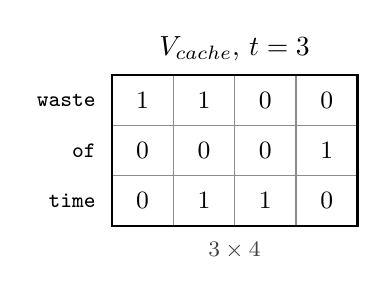
\begin{tikzpicture}
\draw[black!45, fill=white] (0.000,0.000) rectangle (0.780,-0.640);
\node[font=\small, text=black] at (0.390,-0.320) {$1$};
\draw[black!45, fill=white] (0.780,0.000) rectangle (1.560,-0.640);
\node[font=\small, text=black] at (1.170,-0.320) {$1$};
\draw[black!45, fill=white] (1.560,0.000) rectangle (2.340,-0.640);
\node[font=\small, text=black] at (1.950,-0.320) {$0$};
\draw[black!45, fill=white] (2.340,0.000) rectangle (3.120,-0.640);
\node[font=\small, text=black] at (2.730,-0.320) {$0$};
\draw[black!45, fill=white] (0.000,-0.640) rectangle (0.780,-1.279);
\node[font=\small, text=black] at (0.390,-0.959) {$0$};
\draw[black!45, fill=white] (0.780,-0.640) rectangle (1.560,-1.279);
\node[font=\small, text=black] at (1.170,-0.959) {$0$};
\draw[black!45, fill=white] (1.560,-0.640) rectangle (2.340,-1.279);
\node[font=\small, text=black] at (1.950,-0.959) {$0$};
\draw[black!45, fill=white] (2.340,-0.640) rectangle (3.120,-1.279);
\node[font=\small, text=black] at (2.730,-0.959) {$1$};
\draw[black!45, fill=white] (0.000,-1.279) rectangle (0.780,-1.919);
\node[font=\small, text=black] at (0.390,-1.599) {$0$};
\draw[black!45, fill=white] (0.780,-1.279) rectangle (1.560,-1.919);
\node[font=\small, text=black] at (1.170,-1.599) {$1$};
\draw[black!45, fill=white] (1.560,-1.279) rectangle (2.340,-1.919);
\node[font=\small, text=black] at (1.950,-1.599) {$1$};
\draw[black!45, fill=white] (2.340,-1.279) rectangle (3.120,-1.919);
\node[font=\small, text=black] at (2.730,-1.599) {$0$};
\draw[line width=0.9pt] (0.000,0.000) rectangle (3.120,-1.919);
\node[anchor=east, font=\footnotesize\ttfamily] at (-0.080,-0.320) {waste};
\node[anchor=east, font=\footnotesize\ttfamily] at (-0.080,-0.959) {of};
\node[anchor=east, font=\footnotesize\ttfamily] at (-0.080,-1.599) {time};
\node[anchor=south, font=\normalsize] at (1.560,0.050) {$V_{\text{cache}}$, $t=3$};
\node[anchor=north, font=\footnotesize, text=black!75] at (1.560,-1.999) {$3\times4$};
\end{tikzpicture}
\qquad
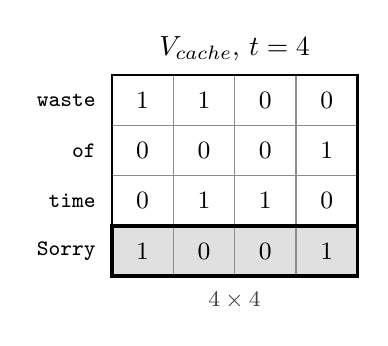
\begin{tikzpicture}
\draw[black!45, fill=white] (0.000,0.000) rectangle (0.780,-0.640);
\node[font=\small, text=black] at (0.390,-0.320) {$1$};
\draw[black!45, fill=white] (0.780,0.000) rectangle (1.560,-0.640);
\node[font=\small, text=black] at (1.170,-0.320) {$1$};
\draw[black!45, fill=white] (1.560,0.000) rectangle (2.340,-0.640);
\node[font=\small, text=black] at (1.950,-0.320) {$0$};
\draw[black!45, fill=white] (2.340,0.000) rectangle (3.120,-0.640);
\node[font=\small, text=black] at (2.730,-0.320) {$0$};
\draw[black!45, fill=white] (0.000,-0.640) rectangle (0.780,-1.279);
\node[font=\small, text=black] at (0.390,-0.959) {$0$};
\draw[black!45, fill=white] (0.780,-0.640) rectangle (1.560,-1.279);
\node[font=\small, text=black] at (1.170,-0.959) {$0$};
\draw[black!45, fill=white] (1.560,-0.640) rectangle (2.340,-1.279);
\node[font=\small, text=black] at (1.950,-0.959) {$0$};
\draw[black!45, fill=white] (2.340,-0.640) rectangle (3.120,-1.279);
\node[font=\small, text=black] at (2.730,-0.959) {$1$};
\draw[black!45, fill=white] (0.000,-1.279) rectangle (0.780,-1.919);
\node[font=\small, text=black] at (0.390,-1.599) {$0$};
\draw[black!45, fill=white] (0.780,-1.279) rectangle (1.560,-1.919);
\node[font=\small, text=black] at (1.170,-1.599) {$1$};
\draw[black!45, fill=white] (1.560,-1.279) rectangle (2.340,-1.919);
\node[font=\small, text=black] at (1.950,-1.599) {$1$};
\draw[black!45, fill=white] (2.340,-1.279) rectangle (3.120,-1.919);
\node[font=\small, text=black] at (2.730,-1.599) {$0$};
\draw[black!45, fill=black!12] (0.000,-1.919) rectangle (0.780,-2.558);
\node[font=\small, text=black] at (0.390,-2.239) {$1$};
\draw[black!45, fill=black!12] (0.780,-1.919) rectangle (1.560,-2.558);
\node[font=\small, text=black] at (1.170,-2.239) {$0$};
\draw[black!45, fill=black!12] (1.560,-1.919) rectangle (2.340,-2.558);
\node[font=\small, text=black] at (1.950,-2.239) {$0$};
\draw[black!45, fill=black!12] (2.340,-1.919) rectangle (3.120,-2.558);
\node[font=\small, text=black] at (2.730,-2.239) {$1$};
\draw[line width=1.4pt] (0.000,-1.919) rectangle (3.120,-2.558);
\draw[line width=0.9pt] (0.000,0.000) rectangle (3.120,-2.558);
\node[anchor=east, font=\footnotesize\ttfamily] at (-0.080,-0.320) {waste};
\node[anchor=east, font=\footnotesize\ttfamily] at (-0.080,-0.959) {of};
\node[anchor=east, font=\footnotesize\ttfamily] at (-0.080,-1.599) {time};
\node[anchor=east, font=\footnotesize\ttfamily] at (-0.080,-2.239) {Sorry};
\node[anchor=south, font=\normalsize] at (1.560,0.050) {$V_{\text{cache}}$, $t=4$};
\node[anchor=north, font=\footnotesize, text=black!75] at (1.560,-2.638) {$4\times4$};
\end{tikzpicture}
\qquad
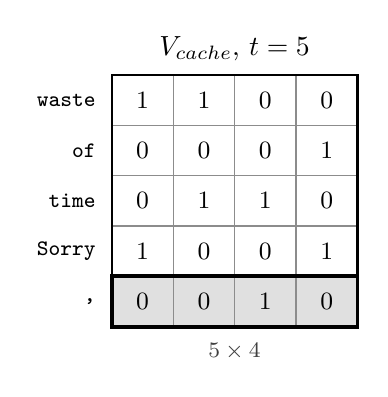
\begin{tikzpicture}
\draw[black!45, fill=white] (0.000,0.000) rectangle (0.780,-0.640);
\node[font=\small, text=black] at (0.390,-0.320) {$1$};
\draw[black!45, fill=white] (0.780,0.000) rectangle (1.560,-0.640);
\node[font=\small, text=black] at (1.170,-0.320) {$1$};
\draw[black!45, fill=white] (1.560,0.000) rectangle (2.340,-0.640);
\node[font=\small, text=black] at (1.950,-0.320) {$0$};
\draw[black!45, fill=white] (2.340,0.000) rectangle (3.120,-0.640);
\node[font=\small, text=black] at (2.730,-0.320) {$0$};
\draw[black!45, fill=white] (0.000,-0.640) rectangle (0.780,-1.279);
\node[font=\small, text=black] at (0.390,-0.959) {$0$};
\draw[black!45, fill=white] (0.780,-0.640) rectangle (1.560,-1.279);
\node[font=\small, text=black] at (1.170,-0.959) {$0$};
\draw[black!45, fill=white] (1.560,-0.640) rectangle (2.340,-1.279);
\node[font=\small, text=black] at (1.950,-0.959) {$0$};
\draw[black!45, fill=white] (2.340,-0.640) rectangle (3.120,-1.279);
\node[font=\small, text=black] at (2.730,-0.959) {$1$};
\draw[black!45, fill=white] (0.000,-1.279) rectangle (0.780,-1.919);
\node[font=\small, text=black] at (0.390,-1.599) {$0$};
\draw[black!45, fill=white] (0.780,-1.279) rectangle (1.560,-1.919);
\node[font=\small, text=black] at (1.170,-1.599) {$1$};
\draw[black!45, fill=white] (1.560,-1.279) rectangle (2.340,-1.919);
\node[font=\small, text=black] at (1.950,-1.599) {$1$};
\draw[black!45, fill=white] (2.340,-1.279) rectangle (3.120,-1.919);
\node[font=\small, text=black] at (2.730,-1.599) {$0$};
\draw[black!45, fill=white] (0.000,-1.919) rectangle (0.780,-2.558);
\node[font=\small, text=black] at (0.390,-2.239) {$1$};
\draw[black!45, fill=white] (0.780,-1.919) rectangle (1.560,-2.558);
\node[font=\small, text=black] at (1.170,-2.239) {$0$};
\draw[black!45, fill=white] (1.560,-1.919) rectangle (2.340,-2.558);
\node[font=\small, text=black] at (1.950,-2.239) {$0$};
\draw[black!45, fill=white] (2.340,-1.919) rectangle (3.120,-2.558);
\node[font=\small, text=black] at (2.730,-2.239) {$1$};
\draw[black!45, fill=black!12] (0.000,-2.558) rectangle (0.780,-3.198);
\node[font=\small, text=black] at (0.390,-2.878) {$0$};
\draw[black!45, fill=black!12] (0.780,-2.558) rectangle (1.560,-3.198);
\node[font=\small, text=black] at (1.170,-2.878) {$0$};
\draw[black!45, fill=black!12] (1.560,-2.558) rectangle (2.340,-3.198);
\node[font=\small, text=black] at (1.950,-2.878) {$1$};
\draw[black!45, fill=black!12] (2.340,-2.558) rectangle (3.120,-3.198);
\node[font=\small, text=black] at (2.730,-2.878) {$0$};
\draw[line width=1.4pt] (0.000,-2.558) rectangle (3.120,-3.198);
\draw[line width=0.9pt] (0.000,0.000) rectangle (3.120,-3.198);
\node[anchor=east, font=\footnotesize\ttfamily] at (-0.080,-0.320) {waste};
\node[anchor=east, font=\footnotesize\ttfamily] at (-0.080,-0.959) {of};
\node[anchor=east, font=\footnotesize\ttfamily] at (-0.080,-1.599) {time};
\node[anchor=east, font=\footnotesize\ttfamily] at (-0.080,-2.239) {Sorry};
\node[anchor=east, font=\footnotesize\ttfamily] at (-0.080,-2.878) {{,}};
\node[anchor=south, font=\normalsize] at (1.560,0.050) {$V_{\text{cache}}$, $t=5$};
\node[anchor=north, font=\footnotesize, text=black!75] at (1.560,-3.278) {$5\times4$};
\end{tikzpicture}
}
\caption{The KV cache growing. After the prompt the cache holds 3 rows; reading \tok{Sorry} adds a
fourth, reading the comma a fifth. Rows are only ever added, never changed, because a token's key
$\bm{x}W_K$ and value $\bm{x}W_V$ depend on nothing but that token.}
\label{fig:ch9grow}
\end{figure}

\paragraph{Worked example: the turn that reads \tok{Sorry}.} The prompt \tok{waste of time} has been read, so the
cache holds the three keys and values of Chapter 3. Now \tok{Sorry} arrives, with arrow $(1,1,0,0)$.

\Predict Before computing: will \tok{Sorry}'s query, $\nNineSorryQ$, agree more with the key of
\tok{waste}, $(0,0,2,2)$, or with the key of \tok{of}, $(1,0,0,0)$? Look at where each has its non-zero
numbers.

\begin{enumerate}[label=\arabic*.,leftmargin=1.6em]
\item New rows. Key $\nNineSorryK$, value $\nNineSorryV$, query $\nNineSorryQ$. Only these three are computed
for this turn.
\item Append the key and value to the cache, which now has 4 rows.
\item Scores: one query row meets the 4 cached keys, stood up as columns ($K_{\text{cache}}^\top$). The
picture below works out the highlighted cell; the other three are the same row meeting a different column.
The scores are $\nNineSorryScores$.
\item Divide by $\sqrt{4}=2$ and apply softmax: shares $\nNineSorryShares$.
\item Mix the cached values with these shares (second picture): $\bm{o}_{\text{Sorry}} = \nNineSorryOut$.
\end{enumerate}
\par\medskip\noindent\begin{minipage}{\linewidth}\centering
\fitR{% AUTO-GENERATED by code/figlib.py helpers -- do not edit
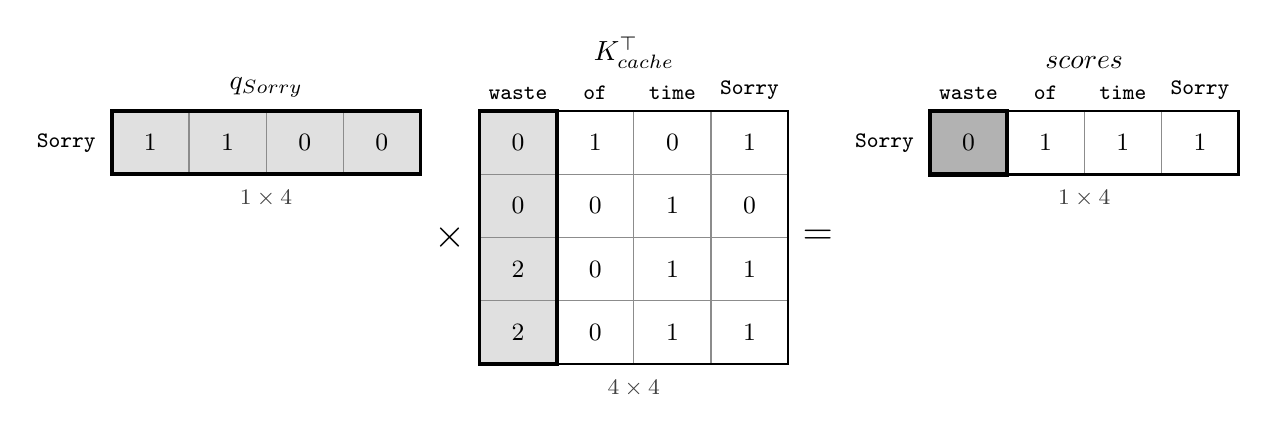
\begin{tikzpicture}
\draw[black!45, fill=black!12] (0.000,0.000) rectangle (0.980,-0.804);
\node[font=\small, text=black] at (0.490,-0.402) {$1$};
\draw[black!45, fill=black!12] (0.980,0.000) rectangle (1.960,-0.804);
\node[font=\small, text=black] at (1.470,-0.402) {$1$};
\draw[black!45, fill=black!12] (1.960,0.000) rectangle (2.940,-0.804);
\node[font=\small, text=black] at (2.450,-0.402) {$0$};
\draw[black!45, fill=black!12] (2.940,0.000) rectangle (3.920,-0.804);
\node[font=\small, text=black] at (3.430,-0.402) {$0$};
\draw[line width=1.4pt] (0.000,0.000) rectangle (3.920,-0.804);
\draw[line width=0.9pt] (0.000,0.000) rectangle (3.920,-0.804);
\node[anchor=east, font=\footnotesize\ttfamily] at (-0.080,-0.402) {Sorry};
\node[anchor=south, font=\normalsize] at (1.960,0.050) {$\bm{q}_{\text{Sorry}}$};
\node[anchor=north, font=\footnotesize, text=black!75] at (1.960,-0.884) {$1\times4$};
\draw[black!45, fill=black!12] (4.670,0.000) rectangle (5.650,-0.804);
\node[font=\small, text=black] at (5.160,-0.402) {$0$};
\draw[black!45, fill=white] (5.650,0.000) rectangle (6.630,-0.804);
\node[font=\small, text=black] at (6.140,-0.402) {$1$};
\draw[black!45, fill=white] (6.630,0.000) rectangle (7.610,-0.804);
\node[font=\small, text=black] at (7.120,-0.402) {$0$};
\draw[black!45, fill=white] (7.610,0.000) rectangle (8.590,-0.804);
\node[font=\small, text=black] at (8.100,-0.402) {$1$};
\draw[black!45, fill=black!12] (4.670,-0.804) rectangle (5.650,-1.607);
\node[font=\small, text=black] at (5.160,-1.205) {$0$};
\draw[black!45, fill=white] (5.650,-0.804) rectangle (6.630,-1.607);
\node[font=\small, text=black] at (6.140,-1.205) {$0$};
\draw[black!45, fill=white] (6.630,-0.804) rectangle (7.610,-1.607);
\node[font=\small, text=black] at (7.120,-1.205) {$1$};
\draw[black!45, fill=white] (7.610,-0.804) rectangle (8.590,-1.607);
\node[font=\small, text=black] at (8.100,-1.205) {$0$};
\draw[black!45, fill=black!12] (4.670,-1.607) rectangle (5.650,-2.411);
\node[font=\small, text=black] at (5.160,-2.009) {$2$};
\draw[black!45, fill=white] (5.650,-1.607) rectangle (6.630,-2.411);
\node[font=\small, text=black] at (6.140,-2.009) {$0$};
\draw[black!45, fill=white] (6.630,-1.607) rectangle (7.610,-2.411);
\node[font=\small, text=black] at (7.120,-2.009) {$1$};
\draw[black!45, fill=white] (7.610,-1.607) rectangle (8.590,-2.411);
\node[font=\small, text=black] at (8.100,-2.009) {$1$};
\draw[black!45, fill=black!12] (4.670,-2.411) rectangle (5.650,-3.214);
\node[font=\small, text=black] at (5.160,-2.813) {$2$};
\draw[black!45, fill=white] (5.650,-2.411) rectangle (6.630,-3.214);
\node[font=\small, text=black] at (6.140,-2.813) {$0$};
\draw[black!45, fill=white] (6.630,-2.411) rectangle (7.610,-3.214);
\node[font=\small, text=black] at (7.120,-2.813) {$1$};
\draw[black!45, fill=white] (7.610,-2.411) rectangle (8.590,-3.214);
\node[font=\small, text=black] at (8.100,-2.813) {$1$};
\draw[line width=1.4pt] (4.670,0.000) rectangle (5.650,-3.214);
\draw[line width=0.9pt] (4.670,0.000) rectangle (8.590,-3.214);
\node[anchor=south, font=\footnotesize\ttfamily] at (5.160,0.020) {waste};
\node[anchor=south, font=\footnotesize\ttfamily] at (6.140,0.020) {of};
\node[anchor=south, font=\footnotesize\ttfamily] at (7.120,0.020) {time};
\node[anchor=south, font=\footnotesize\ttfamily] at (8.100,0.020) {Sorry};
\node[anchor=south, font=\normalsize] at (6.630,0.420) {$K_{\text{cache}}^\top$};
\node[anchor=north, font=\footnotesize, text=black!75] at (6.630,-3.294) {$4\times4$};
\draw[black!45, fill=black!30] (10.390,0.000) rectangle (11.370,-0.804);
\node[font=\small, text=black] at (10.880,-0.402) {$0$};
\draw[black!45, fill=white] (11.370,0.000) rectangle (12.350,-0.804);
\node[font=\small, text=black] at (11.860,-0.402) {$1$};
\draw[black!45, fill=white] (12.350,0.000) rectangle (13.330,-0.804);
\node[font=\small, text=black] at (12.840,-0.402) {$1$};
\draw[black!45, fill=white] (13.330,0.000) rectangle (14.310,-0.804);
\node[font=\small, text=black] at (13.820,-0.402) {$1$};
\draw[line width=1.6pt] (10.390,0.000) rectangle (11.370,-0.804);
\draw[line width=0.9pt] (10.390,0.000) rectangle (14.310,-0.804);
\node[anchor=east, font=\footnotesize\ttfamily] at (10.310,-0.402) {Sorry};
\node[anchor=south, font=\footnotesize\ttfamily] at (10.880,0.020) {waste};
\node[anchor=south, font=\footnotesize\ttfamily] at (11.860,0.020) {of};
\node[anchor=south, font=\footnotesize\ttfamily] at (12.840,0.020) {time};
\node[anchor=south, font=\footnotesize\ttfamily] at (13.820,0.020) {Sorry};
\node[anchor=south, font=\normalsize] at (12.350,0.420) {$\text{scores}$};
\node[anchor=north, font=\footnotesize, text=black!75] at (12.350,-0.884) {$1\times4$};
\node[font=\Large] at (4.295,-1.607) {$\times$};
\node[font=\Large] at (8.965,-1.607) {$=$};
\end{tikzpicture}
}\\[2pt]
% AUTO-GENERATED by code/ch*_figs.py -- do not edit
{\small highlighted row (\texttt{Sorry}'s query) $\cdot$ highlighted column (\texttt{waste}'s key): $(1)(0) + (1)(0) + (0)(2) + (0)(2) = \mathbf{0}$}
\\[10pt]
\fitR{% AUTO-GENERATED by code/figlib.py helpers -- do not edit
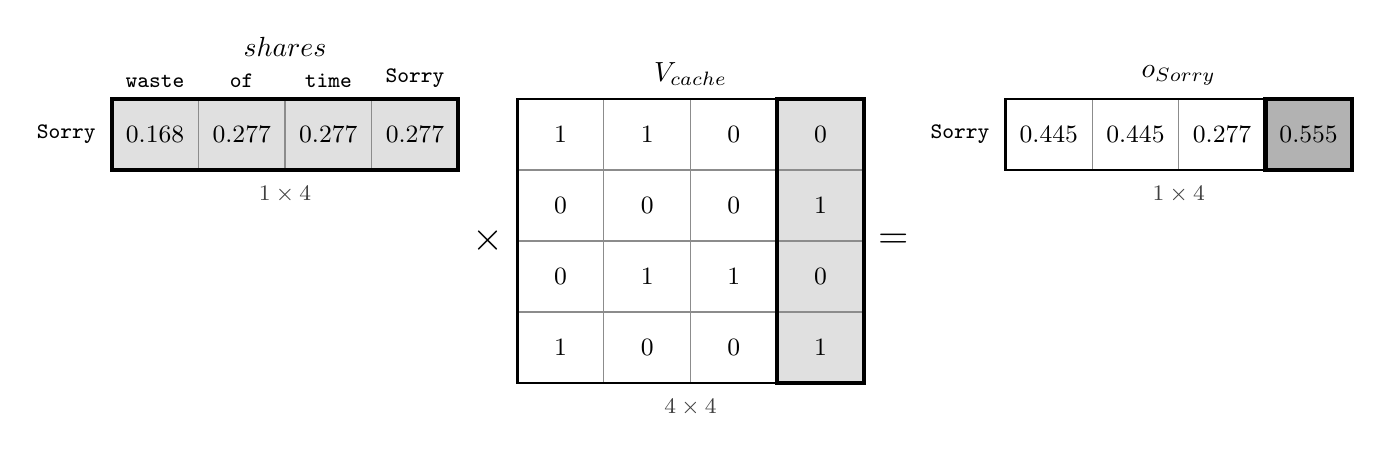
\begin{tikzpicture}
\draw[black!45, fill=black!12] (0.000,0.000) rectangle (1.100,-0.902);
\node[font=\small, text=black] at (0.550,-0.451) {$0.168$};
\draw[black!45, fill=black!12] (1.100,0.000) rectangle (2.200,-0.902);
\node[font=\small, text=black] at (1.650,-0.451) {$0.277$};
\draw[black!45, fill=black!12] (2.200,0.000) rectangle (3.300,-0.902);
\node[font=\small, text=black] at (2.750,-0.451) {$0.277$};
\draw[black!45, fill=black!12] (3.300,0.000) rectangle (4.400,-0.902);
\node[font=\small, text=black] at (3.850,-0.451) {$0.277$};
\draw[line width=1.4pt] (0.000,0.000) rectangle (4.400,-0.902);
\draw[line width=0.9pt] (0.000,0.000) rectangle (4.400,-0.902);
\node[anchor=east, font=\footnotesize\ttfamily] at (-0.080,-0.451) {Sorry};
\node[anchor=south, font=\footnotesize\ttfamily] at (0.550,0.020) {waste};
\node[anchor=south, font=\footnotesize\ttfamily] at (1.650,0.020) {of};
\node[anchor=south, font=\footnotesize\ttfamily] at (2.750,0.020) {time};
\node[anchor=south, font=\footnotesize\ttfamily] at (3.850,0.020) {Sorry};
\node[anchor=south, font=\normalsize] at (2.200,0.420) {$\text{shares}$};
\node[anchor=north, font=\footnotesize, text=black!75] at (2.200,-0.982) {$1\times4$};
\draw[black!45, fill=white] (5.150,0.000) rectangle (6.250,-0.902);
\node[font=\small, text=black] at (5.700,-0.451) {$1$};
\draw[black!45, fill=white] (6.250,0.000) rectangle (7.350,-0.902);
\node[font=\small, text=black] at (6.800,-0.451) {$1$};
\draw[black!45, fill=white] (7.350,0.000) rectangle (8.450,-0.902);
\node[font=\small, text=black] at (7.900,-0.451) {$0$};
\draw[black!45, fill=black!12] (8.450,0.000) rectangle (9.550,-0.902);
\node[font=\small, text=black] at (9.000,-0.451) {$0$};
\draw[black!45, fill=white] (5.150,-0.902) rectangle (6.250,-1.804);
\node[font=\small, text=black] at (5.700,-1.353) {$0$};
\draw[black!45, fill=white] (6.250,-0.902) rectangle (7.350,-1.804);
\node[font=\small, text=black] at (6.800,-1.353) {$0$};
\draw[black!45, fill=white] (7.350,-0.902) rectangle (8.450,-1.804);
\node[font=\small, text=black] at (7.900,-1.353) {$0$};
\draw[black!45, fill=black!12] (8.450,-0.902) rectangle (9.550,-1.804);
\node[font=\small, text=black] at (9.000,-1.353) {$1$};
\draw[black!45, fill=white] (5.150,-1.804) rectangle (6.250,-2.706);
\node[font=\small, text=black] at (5.700,-2.255) {$0$};
\draw[black!45, fill=white] (6.250,-1.804) rectangle (7.350,-2.706);
\node[font=\small, text=black] at (6.800,-2.255) {$1$};
\draw[black!45, fill=white] (7.350,-1.804) rectangle (8.450,-2.706);
\node[font=\small, text=black] at (7.900,-2.255) {$1$};
\draw[black!45, fill=black!12] (8.450,-1.804) rectangle (9.550,-2.706);
\node[font=\small, text=black] at (9.000,-2.255) {$0$};
\draw[black!45, fill=white] (5.150,-2.706) rectangle (6.250,-3.608);
\node[font=\small, text=black] at (5.700,-3.157) {$1$};
\draw[black!45, fill=white] (6.250,-2.706) rectangle (7.350,-3.608);
\node[font=\small, text=black] at (6.800,-3.157) {$0$};
\draw[black!45, fill=white] (7.350,-2.706) rectangle (8.450,-3.608);
\node[font=\small, text=black] at (7.900,-3.157) {$0$};
\draw[black!45, fill=black!12] (8.450,-2.706) rectangle (9.550,-3.608);
\node[font=\small, text=black] at (9.000,-3.157) {$1$};
\draw[line width=1.4pt] (8.450,0.000) rectangle (9.550,-3.608);
\draw[line width=0.9pt] (5.150,0.000) rectangle (9.550,-3.608);
\node[anchor=south, font=\normalsize] at (7.350,0.050) {$V_{\text{cache}}$};
\node[anchor=north, font=\footnotesize, text=black!75] at (7.350,-3.688) {$4\times4$};
\draw[black!45, fill=white] (11.350,0.000) rectangle (12.450,-0.902);
\node[font=\small, text=black] at (11.900,-0.451) {$0.445$};
\draw[black!45, fill=white] (12.450,0.000) rectangle (13.550,-0.902);
\node[font=\small, text=black] at (13.000,-0.451) {$0.445$};
\draw[black!45, fill=white] (13.550,0.000) rectangle (14.650,-0.902);
\node[font=\small, text=black] at (14.100,-0.451) {$0.277$};
\draw[black!45, fill=black!30] (14.650,0.000) rectangle (15.750,-0.902);
\node[font=\small, text=black] at (15.200,-0.451) {$0.555$};
\draw[line width=1.6pt] (14.650,0.000) rectangle (15.750,-0.902);
\draw[line width=0.9pt] (11.350,0.000) rectangle (15.750,-0.902);
\node[anchor=east, font=\footnotesize\ttfamily] at (11.270,-0.451) {Sorry};
\node[anchor=south, font=\normalsize] at (13.550,0.050) {$\bm{o}_{\text{Sorry}}$};
\node[anchor=north, font=\footnotesize, text=black!75] at (13.550,-0.982) {$1\times4$};
\node[font=\Large] at (4.775,-1.804) {$\times$};
\node[font=\Large] at (9.925,-1.804) {$=$};
\end{tikzpicture}
}\\[2pt]
% AUTO-GENERATED by code/ch*_figs.py -- do not edit
{\small highlighted row (the shares) $\cdot$ highlighted column (column 4 of $V_{\text{cache}}$): $(0.168)(0) + (0.277)(1) + (0.277)(0) + (0.277)(1) = \mathbf{0.555}$}

\captionof{figure}{The turn that reads \tok{Sorry}, as two products. Top: the one new query times the
transposed key cache gives one row of 4 scores. Bottom: the 4 shares times the value cache give the output.
Shapes: $(1\times4)(4\times4)=1\times4$ both times. Nothing here is $4\times4$ work on the old tokens.}
\end{minipage}\par\medskip

\tok{waste} gets the smallest share here: \tok{Sorry}'s query points along the first two directions, where
\tok{waste}'s key has nothing. (Did your prediction hold?)

\Sanity We ran the whole reply both ways: the full recompute of Chapter 3 on every turn, and the cache.
The largest difference between any output number of the two methods, over all \nNineSteps\ turns, was
\nNineMaxDiff. Not small: zero. The cache is not an approximation. It does the same arithmetic, and skips only
arithmetic whose result it already has.

\begin{breaks}
A librarian's card can go out of date if the book is edited. A cached key cannot: once a token is written,
its arrow and the weights never change during the reply. The picture breaks the other way too: the cards
take up shelf space, and in \S9.5 that shelf turns out to be the main cost.
\end{breaks}

\Why Why cache keys and values, and not queries? A query is only used on the turn its token arrives, to
ask its one question. Keys and values are used by every \emph{later} token. What is reused is worth
storing; what is used once is not. Remember the question from Chapter 3, why does \tok{time} need a key and a
value of its own? Here is the second half of the answer: so that every token after it can find it and read it.

\begin{wrongidea}{9.3}
``The cache must also store the queries.'' It is tempting because $Q$, $K$ and $V$ are made together. But
look at the formula: old queries never appear in it. The only query on a turn is the newest one.
\end{wrongidea}

\begin{checkq}
After the cache is added, the toy's outputs change from $\oTime$ to something else for \tok{time}. What
went wrong, if anything?
\begin{options}
\item Nothing; a cache always changes outputs a little.
\item Something is broken: with a correct cache the outputs are identical.
\item The cache was missing the queries.
\item The prompt is too short for a cache to be accurate.
\end{options}
\end{checkq}

\Summary{The KV cache keeps every earlier token's key and value, so each turn computes one new query, key and
value and one row of scores, and gets exactly the same answer.}

%---------------------------------------------------------------------
\subsection*{9.4\quad Two phases: prefill and decode}

Generation has two phases with very different shapes.

\Picture A shop opening for the day. In the morning delivery (\emph{prefill}) a whole lorry of boxes is
unloaded at once, many hands working in parallel. After that, customers come one at a time
(\emph{decode}), and each one needs the shopkeeper to walk the whole shop.

\Exactly \emph{Prefill} reads the prompt: all prompt tokens go through the model together, as in training,
and their keys and values fill the cache. This is big matrix times big matrix, the work GPUs love
(\S3.9). \emph{Decode} writes the reply: one token per turn, so every weight matrix is multiplied by a
single row. For each new token the hardware must read \emph{all} the weights and the whole cache from
memory, and do only a little arithmetic with each number it reads.

How little? Take Qwen3-0.6B (Chapter 10). One decode step does about $2N \approx \nNineQwenDecodeFlops$
billion multiply-adds and must read the weights, about \nNineQwenWeightsGiB\ GiB in fp16. That is roughly
\nNineQwenDecodeIntensity\ arithmetic operation per byte read. A modern GPU can do dozens to hundreds of
operations in the time it reads one byte from its main memory. So during decode the arithmetic units mostly
wait for memory. Decode speed is set by how many bytes must be read per token, and the cache is part of
those bytes.

\begin{wrongidea}{9.4}
``What a model costs to run is set by its weights alone; context length is free.'' The number in a model's name
is its weight count, so it is the number everyone quotes. But whether a model fits on a GPU, a laptop
or a phone depends on the weights \emph{and} on how many tokens of conversation it must hold, as the next
section shows.
\end{wrongidea}

\Summary{Prefill is parallel and arithmetic-heavy; decode goes one token at a time and is limited by how many bytes
it must read, cache included.}

%---------------------------------------------------------------------
\subsection*{9.5\quad The bill}

\Predict A model has 28 layers. Each layer keeps a key and a value per token, for 8 heads of width 128,
each number in 2 bytes. How much memory for one token of conversation? Guess an order of magnitude: bytes,
kilobytes, megabytes?

\Exactly For every token, every layer stores one key and one value per key-value head:
\[
\text{KV bytes} = 2 \times \text{layers} \times \text{kv heads} \times \text{head width} \times \text{tokens}
\times \text{bytes per number}.
\]
The 2 counts K and V. Drawn as a product, for Qwen3-0.6B:

\par\medskip\noindent\begin{minipage}{\linewidth}\centering
\fitR{% AUTO-GENERATED by code/ch*_figs.py -- do not edit
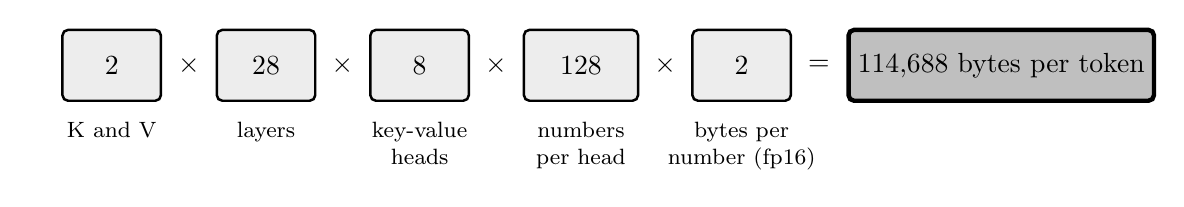
\begin{tikzpicture}[font=\normalsize]
\node[draw, line width=0.9pt, rounded corners=2pt, minimum width=1.25cm, minimum height=0.9cm, fill=black!7] (f0) at (0.62,0) {$2$};
\node[font=\footnotesize, text width=1.9cm, align=center, anchor=north] at (0.62,-0.6) {K and V};
\node at (1.60,0) {$\times$};
\node[draw, line width=0.9pt, rounded corners=2pt, minimum width=1.25cm, minimum height=0.9cm, fill=black!7] (f1) at (2.58,0) {$28$};
\node[font=\footnotesize, text width=1.9cm, align=center, anchor=north] at (2.58,-0.6) {layers};
\node at (3.55,0) {$\times$};
\node[draw, line width=0.9pt, rounded corners=2pt, minimum width=1.25cm, minimum height=0.9cm, fill=black!7] (f2) at (4.53,0) {$8$};
\node[font=\footnotesize, text width=1.9cm, align=center, anchor=north] at (4.53,-0.6) {key-value heads};
\node at (5.50,0) {$\times$};
\node[draw, line width=0.9pt, rounded corners=2pt, minimum width=1.45cm, minimum height=0.9cm, fill=black!7] (f3) at (6.58,0) {$128$};
\node[font=\footnotesize, text width=1.9cm, align=center, anchor=north] at (6.58,-0.6) {numbers per head};
\node at (7.65,0) {$\times$};
\node[draw, line width=0.9pt, rounded corners=2pt, minimum width=1.25cm, minimum height=0.9cm, fill=black!7] (f4) at (8.62,0) {$2$};
\node[font=\footnotesize, text width=1.9cm, align=center, anchor=north] at (8.62,-0.6) {bytes per number (fp16)};
\node at (9.60,0) {$=$};
\node[draw, line width=1.6pt, rounded corners=2pt, minimum height=0.9cm, fill=black!25, anchor=west] at (9.95,0) {$114{,}688$ bytes per token};
\end{tikzpicture}
}
\captionof{figure}{The KV-cache bill for one token of conversation in Qwen3-0.6B. Change any one box and
the bill changes in proportion; \S9.6 shrinks the third box.}
\end{minipage}\par\medskip

\noindent For Qwen3-0.6B that is $2\times28\times8\times128\times2 = \nNineQwenPerTok$ bytes,
about \nNineQwenPerTokKiB\ KiB \emph{per token}. GPT-2 small (12 layers, 12 heads of 64) needs
\nNineGptPerTok\ bytes, \nNineGptPerTokKiB\ KiB. Our script computes the same formula as the calculator
\texttt{code/calc.py}:

\begin{center}
\small
\begin{tabular}{@{}l r r r r@{}}
\toprule
model & weights (fp16) & cache, 1{,}024 tokens & 8{,}192 tokens & 32{,}768 tokens\\
\midrule
GPT-2 small & \nNineGptWeightsGiB\ GiB & \nNineGptKvOne\ GiB & \nNineGptKvEight\ GiB$^*$ & \nNineGptKvThirtyTwo\ GiB$^*$\\
Qwen3-0.6B & \nNineQwenWeightsGiB\ GiB & \nNineQwenKvOne\ GiB & \nNineQwenKvEight\ GiB & \nNineQwenKvThirtyTwo\ GiB\\
\bottomrule
\end{tabular}

{\footnotesize $^*$GPT-2 cannot read past 1{,}024 tokens; these columns show what the same design would cost.}
\end{center}

Read the Qwen row. At about \nNineQwenCross\ tokens of conversation, the cache is as large as the whole
model. At 32{,}768 tokens it is three times the model. And this is for \emph{one} conversation: a server
answering 16 such conversations at once needs \nNineQwenBatchSixteen\ GiB of cache. For long conversations,
the bill is the cache.

\Why The cache trades memory for arithmetic. That trade was a bargain in \S9.2, and it stays a bargain, but
memory is the scarce thing on a GPU and the cache grows with every token. So the next ideas all attack the
same formula: fewer layers, fewer key-value heads, narrower heads, or fewer bytes per number. Which of those
would you touch first, and what would each cost you?

\begin{checkq}
You double the context from 8{,}192 to 16{,}384 tokens. What happens to Qwen3-0.6B's cache?
\begin{options}
\item It doubles.
\item It quadruples, because attention is quadratic in length.
\item It stays the same; the cache size is fixed by the weights.
\item It grows a little, because only new tokens are added.
\end{options}
\end{checkq}

\Summary{The cache costs $2\times\text{layers}\times\text{kv heads}\times\text{head width}\times\text{bytes}$ per token,
and for long conversations it outgrows the model itself.}

%---------------------------------------------------------------------
\subsection*{9.6\quad Paying less: sharing keys and values between heads}

Chapter 5 gave each attention head its own queries, keys and values. In the formula above, the number of
\emph{key-value} heads is what matters. What if several query heads shared one set of keys and values?

\Picture A class of 16 students each asking their own question, but sharing 8 textbooks instead of
carrying 16. Every student still asks what they want; they read the answers from shared books.

\Exactly \emph{Multi-query attention} (Shazeer, 2019) keeps all the query heads but gives the whole layer a
single key head and a single value head. \emph{Grouped-query attention} (Ainslie et al., 2023) sits in
between: query heads are split into groups, and each group shares one key head and one value head.
Qwen3-0.6B uses 16 query heads and 8 key-value heads, so each pair of query heads shares its keys and values.
For 32{,}768 tokens:

\begin{center}
\small
\begin{tabular}{@{}l r r@{}}
\toprule
Qwen3-0.6B with \ldots & key-value heads & cache at 32{,}768 tokens\\
\midrule
full multi-head attention & 16 & \nNineQwenMhaThirtyTwo\ GiB\\
grouped-query attention (what it uses) & 8 & \nNineQwenKvThirtyTwo\ GiB\\
multi-query attention & 1 & \nNineQwenMqaThirtyTwo\ GiB\\
\bottomrule
\end{tabular}
\end{center}

\begin{breaks}
Students sharing a book all read the same pages. Heads sharing keys and values all see the same ``labels''
and the same ``contents'' for every token; only their questions differ. Something is lost: fewer independent
ways to describe each token. Ainslie and colleagues found that grouping kept quality close to full multi-head
attention while multi-query lost more; how much is lost is an empirical question for each model, not a law.
\end{breaks}

\begin{wrongidea}{9.5}
``Fewer key-value heads means the model looks at fewer things.'' The number of \emph{ways of asking} is the
number of query heads, and that is unchanged. What shrinks is the number of independent ways each token can
be found and read.
\end{wrongidea}

\Summary{Grouped-query attention lets several query heads share one key and value head, halving Qwen3's cache
compared with full multi-head attention at little cost in quality.}

%---------------------------------------------------------------------
\subsection*{9.7\quad Never writing the big table: FlashAttention}

The cache is about memory that \emph{stays}. There is a second memory cost, during prefill and training:
the $T\times T$ score table of \S3.4. At 32{,}768 tokens, one head in one layer has
\nNineScoreEntries\ billion scores, \nNineScoreGiB\ GiB in fp16, before softmax has even been applied.

\Picture You need the total of a long column of numbers written in a ledger in the basement. One way: carry
each page upstairs, copy it into a giant table on your desk, then add. Another: go down once, add each page
as you read it, and carry up only the running total.

\Exactly FlashAttention (Dao et al., 2022) computes attention in tiles: a block of queries meets a block
of keys inside the GPU's small fast memory, the softmax is kept as a running sum, and the full $T\times T$
table is never written to the large slow memory. The arithmetic is the same and the result is exact (up to
floating-point rounding). What changes is the number of bytes moved, and in \S9.4 we saw that bytes moved are
what limit speed.

\Summary{FlashAttention gets the same answer while never writing the full score table to slow memory.}

\begin{principle}{pay once, reuse; and move fewer bytes}
The KV cache is \emph{memoisation}: store a result that will be asked for again, so you pay for it once.
It works here for a precise reason: the causal mask guarantees that old results never change. Before you cache
anything in a system you build, ask the same question: what guarantees the stored answer is still right? Agent
platforms use the same trade when they cache a long system prompt across calls, and a memory system makes it
when it stores a summary instead of rereading a whole conversation. The second lesson, from \S9.4 and
\S9.7, transfers too: when a system is slow, count the bytes it moves before counting the arithmetic it does.
\end{principle}

\begin{lookingback}
\begin{enumerate}[label=\arabic*.,leftmargin=1.6em]
\item (Chapter 3) Why does the causal mask guarantee that earlier tokens' outputs do not change when a new
token is appended?
\item (Chapter 1) Hallucination was described as a consequence of writing one token at a time. Does the KV
cache make it more likely, less likely, or neither? Why?
\end{enumerate}
\end{lookingback}

%---------------------------------------------------------------------
\subsection*{Exercises}

\begin{exercise}
Using the formula of \S9.5, compute GPT-2 small's cache for one conversation of 1{,}024 tokens in fp16.
Then compute it again with numbers stored in 1 byte each (8-bit). Check the first against the table.
\end{exercise}

\begin{exercise}
(Fading worked example.) The turn after \tok{Sorry} reads the token \tok{,} with arrow $(0,0,0,1)$. Fill in the
gaps: its key is $(0,0,0,1)W_K = (\underline{\quad},\underline{\quad},\underline{\quad},\underline{\quad})$;
the cache now has \underline{\quad} rows; its query is $(0,0,0,1)$, so its score against each cached key is
that key's \underline{\quad}-th entry.
\end{exercise}

\begin{exercise}
A model has 32 layers, 32 query heads, 8 key-value heads and head width 128. A product team wants 100
simultaneous conversations of 8{,}192 tokens in fp16. How much cache memory is that? What would it be with
full multi-head attention?
\end{exercise}

\begin{exercise}
Explain to a friend, in three sentences and without symbols, why decode is limited by memory rather than
arithmetic.
\end{exercise}

%---------------------------------------------------------------------
\subsection*{Answers to Chapter 9}

\paragraph{Check yourself 9.1.} (b). With a correct cache the outputs are identical; our script measured a
largest difference of \nNineMaxDiff. (a) is misconception M9.2, the cache as a lossy shortcut. (c) is M9.3: old
queries are never used. (d) treats the cache as an approximation that needs enough data; it is not an
approximation at all.

\paragraph{Check yourself 9.2.} (a). The cache has one row per token per layer per head, so it grows in
proportion to length. (b) confuses the cache with the score table, which is $T\times T$ (\S9.7). (c) is
M9.4. (d) is true per token added but the cache still ends up twice as large.

\paragraph{Looking back.} (1) Each earlier token's row of the score table has $-\infty$ in every position to its
right, so a new token is invisible to it; its shares and output are unchanged. (2) Neither: the cache gives
exactly the same outputs as recomputing, so it changes nothing about what is written.

\paragraph{Exercise 9.1.} $2\times12\times12\times64\times1{,}024\times2 = \nNineExOne$ bytes $=$ \nNineExOneMiB\ MiB,
which the table rounds to \nNineGptKvOne\ GiB. With 1 byte per number, half: \nNineExOneHalfMiB\ MiB.

\paragraph{Exercise 9.2.} Row 4 of $W_K$ is the key: $\nNineCommaK$. The cache has 5 rows.
The query $(0,0,0,1)$ picks the 4th entry of each key. The cached keys are $(0,0,2,2)$, $(1,0,0,0)$,
$(0,1,1,1)$, $\nNineSorryK$ and $\nNineCommaK$, so the scores are $\nNineCommaScores$.

\paragraph{Exercise 9.3.} Per token: $2\times32\times8\times128\times2 = \nNineExThreeTok$ bytes $=$ \nNineExThreeTokKiB\ KiB. Times
$8{,}192$ tokens and 100 conversations: $\nNineExThreeTot$ bytes $=$ \nNineExThreeGiB\ GiB. With 32 key-value heads,
four times as much: \nNineExThreeMhaGiB\ GiB.

\paragraph{Exercise 9.4.} One possible answer: to write each word, the computer has to fetch every number in
the model and the whole conversation so far from its memory. It then does only about one sum with each number.
Its calculators are far faster than its memory, so they spend most of the time waiting for numbers to arrive.

\subsection*{What you now know}
\begin{itemize}
\item Writing a reply is a loop, and almost all of the work in it would be repeated without a cache.
\item The KV cache stores each token's key and value; each turn computes one query and one row of scores, and the
outputs are exactly the same.
\item Prefill is parallel; decode is one token at a time and limited by bytes read.
\item The cache costs $2\times\text{layers}\times\text{kv heads}\times\text{head width}\times\text{bytes}$
per token: \nNineQwenPerTokKiB\ KiB for Qwen3-0.6B, larger than the model after about \nNineQwenCross\ tokens.
\item Grouped- and multi-query attention shrink the cache by sharing keys and values; FlashAttention avoids
writing the score table to slow memory.
\end{itemize}
